%-----------------------------------LICENSE------------------------------------%
%   This file is part of tikz_figures.                                         %
%                                                                              %
%   tikz_figures is free software: you can redistribute it and/or              %
%   modify it it under the terms of the GNU General Public License as          %
%   published by the Free Software Foundation, either version 3 of the         %
%   License, or (at your option) any later version.                            %
%                                                                              %
%   tikz_figures is distributed in the hope that it will be useful,            %
%   but WITHOUT ANY WARRANTY; without even the implied warranty of             %
%   MERCHANTABILITY or FITNESS FOR A PARTICULAR PURPOSE.  See the              %
%   GNU General Public License for more details.                               %
%                                                                              %
%   You should have received a copy of the GNU General Public License along    %
%   with tikz_figures.  If not, see <https://www.gnu.org/licenses/>.           %
%------------------------------------------------------------------------------%

% Use the standalone class for displaying the tikz image on a small PDF.
\documentclass[crop, tikz]{standalone}

% Import the tikz package to use for the drawing.
\usepackage{tikz}

% Begin the document.
\begin{document}

    % Draw the figure.
    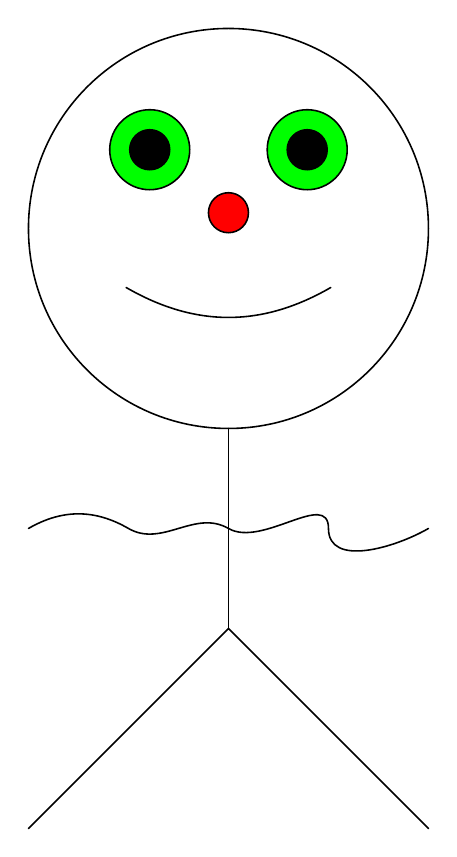
\begin{tikzpicture}[%
        line width = 0.2mm,
        line cap = round
    ]
        % Coordinates for parts of the face.
        \coordinate (Nose) at (0.0, 0.2);
        \coordinate (Right_Eye) at (1.0, 1.0);
        \coordinate (Left_Eye) at (-1.0, 1.0);
        \coordinate (Center) at (0.0, 0.0);

        % Left and right endpoints for the smile.
        \coordinate (Left_Smile) at (210:1.5);
        \coordinate (Right_Smile) at (330:1.5);

        % Circle for the head.
        \draw (Center) circle (1in);

        % Draw in the eyes.
        \draw[fill = green] (Right_Eye) circle (0.2in);
        \draw[fill = green] (Left_Eye) circle (0.2in);
        \draw[fill = black] (Right_Eye) circle (0.1in);
        \draw[fill = black] (Left_Eye) circle (0.1in);
        \draw[fill = red] (Nose) circle (0.1in);

        % Curve for the smile.
        \draw (Left_Smile) to[out = -30, in = -150] (Right_Smile);

        % Straight line for the body.
        \draw (0, -1in) to (0, -2in);

        % V shape for the legs.
        \draw (-1in, -3in) to (0, -2in) to (1in, -3in);

        % Squiggly curve for the arms.
        \draw (-1in, -1.5in)
            to[out = +30, in = +150] (-0.5in, -1.5in)
            to[out = -30, in = +150] (+0.0in, -1.5in)
            to[out = -30, in = +90] (+0.5in, -1.5in)
            to[out = -90, in = -150] (+1.0in, -1.5in);
    \end{tikzpicture}
\end{document}
